\section{Incident life-cycle}
\label{incident-life-cycle}

In \CompanyX{}, an incident is defined as an unplanned interruption or degradation of a product or service that is causing customer impact. For example, a slow connection, a timeout, a crash etc. could constitute an incident. The core part of our paper is to understand the incident management process which defines the various steps an incident goes through – from creation to closing. Bugs and incidents are very different as in our case incidents may or may not lead to bugs. Furthermore, incidents often require the involvement of developers on-call who have been designated to respond to incidents. Figure \ref{fig:incident-lifecycle} presents a high level view of the incident management process. Most online services have their own specific incident management protocol. This figure is a generic process that should apply outside of \CompanyX{} as well.

\begin{figure}[H]
\vspace{-6pt}
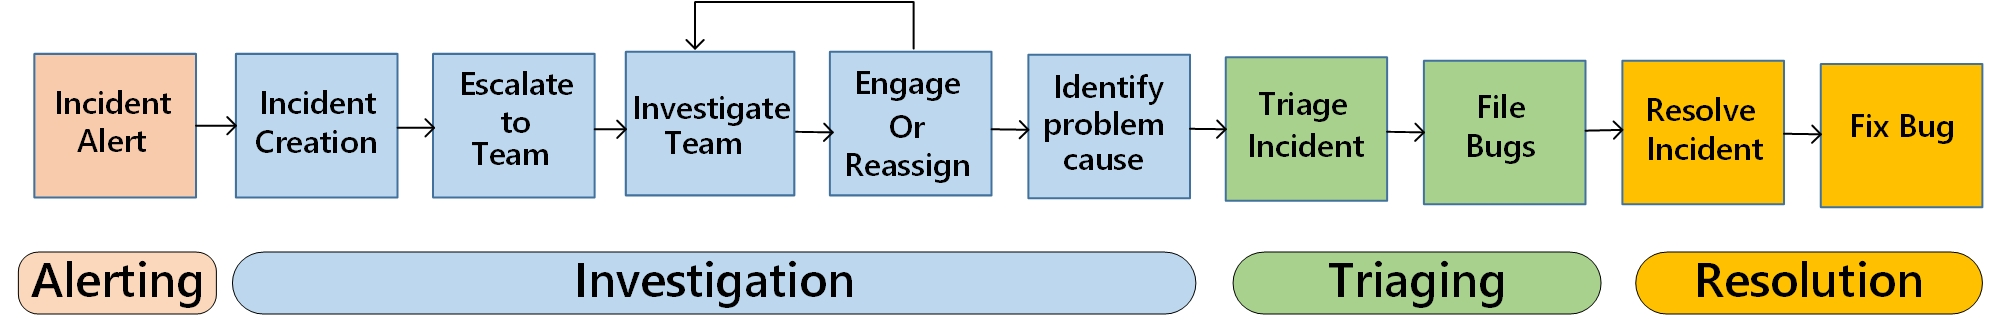
\includegraphics[width=\linewidth]{Figures/Incident_Lifecycle.jpg}
\caption{Incident Life-Cycle}
\label{fig:incident-lifecycle}
\vspace{-6pt}
\end{figure}
The incident management process is broadly classified into 4 phases. In the first phase which is the \emph{alerting} phase, typically an alert is fired when the service monitoring metrics fall below a pre-definitely acceptance level in terms of performance (for example slow response), slow transfer rate, system hang or crash, etc. This leads to phase 2 which is the \emph{investigation} phase. In the investigation phase, firstly an incident is created in the incident database. This is then escalated to a “related” team. The identification of the first “related” team is automatic, based on heuristics or component ownership. The team investigates the incidents and engages with relevant stakeholders or re-routes it to the appropriate team to repeat the steps. 
    
Our work applies directly in the engagement and problem identification phase dealing with unsupervised knowledge extraction from service incidents to aid in the problem resolution. Then the appropriate team identifies the problem cause and moves over to the next phase, which is called \emph{triaging}. In this phase, the incident is triaged according to priority and the appropriate bugs for fixing the incident are filed for the engineering teams to fix. In the final phase of \emph{resolution}, the incident is resolved and the bug is fixed in the system. There are other activities including root cause analysis which happen outside of this timeline in parallel in order to ensure that incidents do not repeat in the future.